% % % % % % % % % % % % % % % % % % % % % % % % % % % % % % % % % % % % % % % % % % % % % % % % %

\newcommand{\reportLanguage}{english}

% % % % % % % % % % % % % % % % % % % % % % % % % % % % % % % % % % % % % % % % % % % % % % % % %



\RequirePackage{fix-cm}
\documentclass[\reportLanguage, twocolumn, 11pt]{article}
%\usepackage{emptypage}
\RequirePackage[l2tabu, orthodox]{nag}
\usepackage[all,error]{onlyamsmath}
\AtBeginDocument{\catcode`$=3 }
\usepackage{fixmath}
%\usepackage{refcheck}
%\ignoreunlbld
\usepackage{todonotes}
\usepackage[backend=biber,
            style=numeric,
            sorting=none
           ]{biblatex}
\usepackage{lipsum}


% --- Mathematical packages ---
\usepackage{amsmath}
\usepackage{amsthm}
\usepackage{amssymb}
\usepackage{bm}
\usepackage[per-mode=fraction,
            exponent-product=\cdot,
            separate-uncertainty=true
           ]{siunitx}
%\usepackage{mathtools}


% --- Typographical packages ---
% - Bases -
\usepackage[utf8]{inputenc}
\usepackage[T1]{fontenc}
\usepackage{babel}
\usepackage[babel]{csquotes}
\usepackage{comment}
% - Font -
\usepackage{newtxtext,newtxmath}
\usepackage[toctitles,compact,explicit]{titlesec}
\usepackage{microtype}
\usepackage{ellipsis}
% - Shape -
\usepackage{setspace}
\usepackage[hyphens]{url}
\usepackage[hidelinks]{hyperref}
\usepackage[noabbrev,capitalise]{cleveref}
\usepackage{fancyhdr}
\usepackage[titles]{tocloft}
%\usepackage{abstract}
\usepackage[margin=2cm]{geometry}

% --- Graphical packages ---
\usepackage{float}
\usepackage{graphicx}
\usepackage{caption}
\usepackage{subcaption}
\usepackage{booktabs}
\usepackage{multirow}


\usepackage{pbox}
% Disable underfull box warnings when breaking URLs
\usepackage{etoolbox}
\apptocmd{\sloppy}{\hbadness 10000\relax}{}{}



\setlength\columnsep{30pt}
\setlength\voffset{1cm}
\addtolength{\textheight}{-2cm}



%%%%%%%%%%%%%%%%%%%%%%%%%%%%%%%%%%%%%%%%%%%%%%%%%%%%%%%%%%%%%%%%%%%%%%
% Edit these according to your needs

\newcommand{\reportType}{Project}

\title{Protein Alignment}

\author{Ernald Shehaj}
\newcommand{\matrNr}{50097030}

\date{}

%%%%%%%%%%%%%%%%%%%%%%%%%%%%%%%%%%%%%%%%%%%%%%%%%%%%%%%%%%%%%%%%%%%%%%



% Generate author and title
\makeatletter



% The literature file
\addbibresource{references.bib}



\newcommand{\reportheader}{Report}
\newcommand{\reportmatriculationnumber}{Matriculation Number}


\graphicspath{{./}}



\begin{document}

{
    \twocolumn[
        \begin{center}
            \LARGE \reportType{} \reportheader: \\ \@title
        \end{center}
        \begin{center}
            \large\@author \\
            \large \reportmatriculationnumber: \matrNr{}
        \end{center}
        \begin{center}
            \large \@date
        \end{center}
        \vspace{0.8cm}
    ]
}
\begin{abstract}
Proteins are large molecular chains that make most biological processes possible\cite{shape}. They make 42\% of the dry weight of the human body, where they can also be found at the cellular level. We study the problem of comparing two or more DNA, RNA, or protein sequences based on their structure\cite{geneious_alignment}. Investigation of protein structure similarities provides information on their functions and dynamics, as well as on the evolutionary relationship between sequences\cite{geneious_alignment}\cite{shape}. In this project, we compare protein structures based solely on C$\alpha$ (alpha carbon). After we construct the feature vectors of each protein that integrate features like nearest-neighbour distances, residue type, secondary structures, and spatial fit, we build a cost matrix that finds the best residue-to-residue correspondence using the Hungarian algorithm. After we obtain optimal amino acid matching, we superpose the matched amino acids using the Kabsch algorithm and find the root-mean-squared-derivation (RMSD) as a quantitive measure of structural stability. After the compilation of the code we get a report of the final RMSD and the coverage, that are defined as the fraction of residues retained after pruning, to capture the quality and extent of the alignment. In addition, a visualization of the matched amino acids side-by-side is given, where the matched amino acids share the same colour. The proteins compared in this project are pig insulin and human insulin. The data that contains the features of one protein is given in a PDB file. A \textbf{PDB (Protein Data Bank) file} is a standardized plain text format for storing 3D structural data of biological macromolecules—chiefly proteins and nucleic acids, as well as their complexes \cite{brasier_pdb_medium}. 
\end{abstract}

% --- Introduction ---
\section{Introduction}
The structures that are responsible for the majority of the processes that make it possible for us to live are proteins. They are responsible for providing structure to cells and tissues, transporting molecules, enabling communication and movement, regulating cellular processes, and protecting the body through the immune system. They are chains of amino acids that have a function, which is determined by the 3D shape they have, therefore, shape matching is essential for understanding their function. Shape matching is the process of comparing two protein chains to identify similarities between residues (amino acids). Amino acids are molecules that serve as the building block for proteins. Figure~\ref{fig:alanine} shows how an amino acid looks like.  
\begin{figure}[h!]
  \centering
  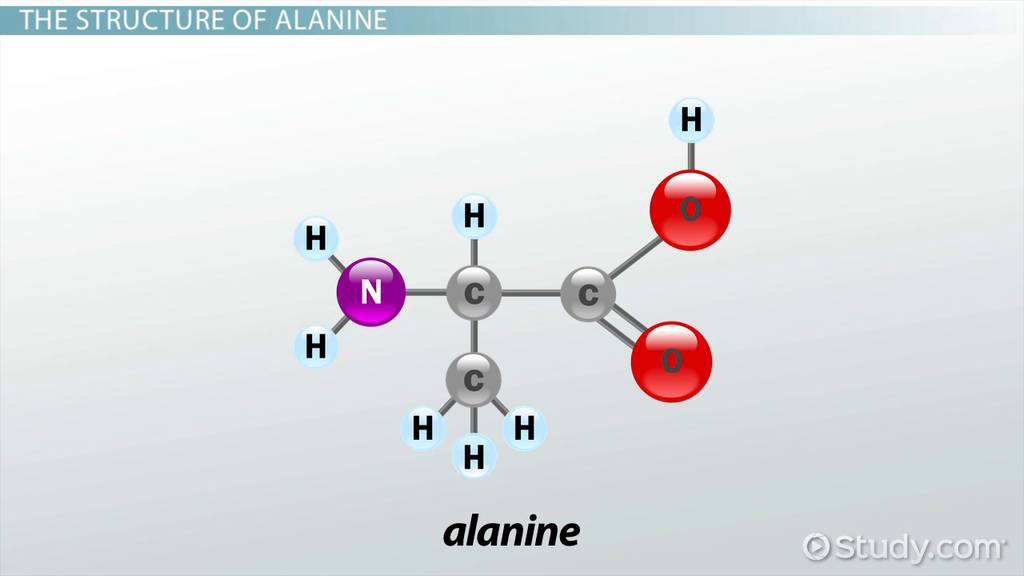
\includegraphics[width=0.4\textwidth]{image.png}
  \caption{Chemical structure of alanine, showing the amino group (purple), carboxyl group (red), and side chain. Adapted from \cite{study_alanine}.}
  \label{fig:alanine}
\end{figure}

The similarities we may recognise while comparing two proteins give hints into: 1) the functional regions of a protein, 2) important structural characteristics of amino acids, 3) the evolutionary relationship between amino acids\cite{geneious_alignment}. The approach that we do in this project is based on the Hungarian algorithm. For every residue(amino acid) we build a feature vector, containing: 1) The C$\alpha$(alpha carbon) distance to the nearest neighbour of one residue, 2) do they contain secondary structures and if yes what do they contain, 3) what is the chemistry of the residue, 4) the distance between amino acids of different proteins using RMSD. We use the Kabsch algorithm to superpose the two structures and compute the root-mean-square deviation (RMSD) in order to have rotation invariance. However there are multiple other methods that we use in order to compare two proteins like: 1) shape retrieval methods based on histograms summarizing local or global geometrical features of the surface shape, 2) shape retrieval methods based on molecular surface maps, i.e. the projection(s) of the protein topography in the 3D space, 3) Feature-based 3D protein alignment\cite{shape}. We compare the human insuline with the insuline mollecule of the pig. The features of each protein mollecule are saved in a pdb file. The files are called respectfully 4nir.pdb and 3nir.pdb.

\section{Related Works}
\subsection{Different categories of methods based on protein alignment}
In order to grasp a better understaning at protein shape matching. We also will present how some other methods work to compare two proteins, given as PDB files.

\textbf{Shape retrieval methods based on histograms summarizing local or global geometrical features of the surface shape} represent protein surfaces by statistical summaries-histograms-of geometric features. These methods are responsible for the computation of descriptors such as distances, curvature, angles, or orientation distributions either globally(enitire surface) or locally(over patches), which result in a histogram that captures the proteins strctural essence. In the proces of comparing two proteins with each other the two histograms are taken and the distance between their descriptors is computed to find how similar they are. This method is computionally efficient and rotation-invariant. In Figure~\ref{fig:placeholder} there is an example of a histogram.\cite{rusu2010vfh}
\begin{figure}
    \centering
    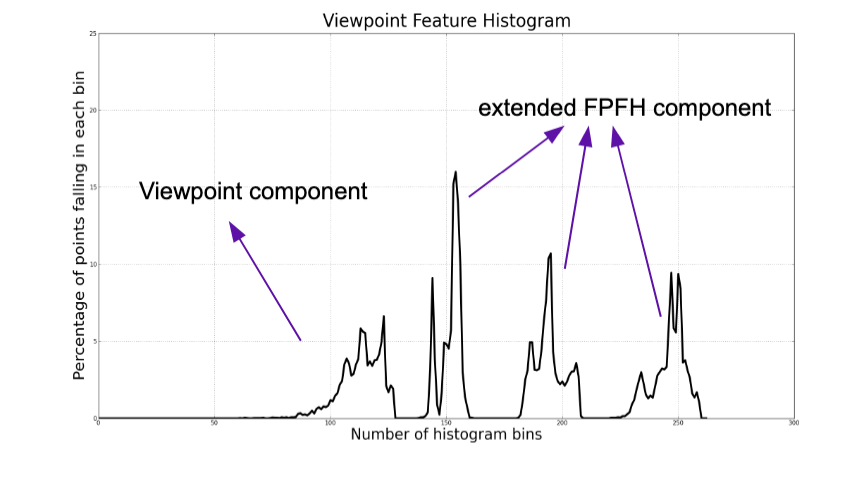
\includegraphics[width=1.0\linewidth]{image1.png}
    \caption{An example of the resultant Viewpoint Feature Histogram for a given object.\cite{rusu2010vfh}}
    \label{fig:placeholder}
\end{figure}

\textbf{Shape retrieval methods based on molecular surface maps, i.e., the projection(s) of the protein topography in the 2D space} tries to represent the molecular surface of a protein  by projecting its 3D topography into a 2D panoramic map. The surface geometry of one object, like a protein, gets "unwrapped", to create a panoramic photo so to say, that captures features like curvature, depth, or surface features. The process works like this that firstly the object gets super-posed, meaning that 
orientation is adjusted so that the object is aligned in a consistent coordinate system. The 3D model in this case the protein gets wrapped by a virtual cylinder. After the wrapping, the surface points are projected onto the cylinder's interior. Then, after the cylinder gets "unfolded" into a 2D surface, the result is a panoramic view of the object's shape. The panoramic view that it produced can be converted into a histogram or even be encoded with descriptors. The comparison than is done by image matching-methods. In Figure~\ref{fig:method2} there is an example of the projection from 3D into a 2D surface of an object.\cite{panorama}
\begin{figure}
    \centering
    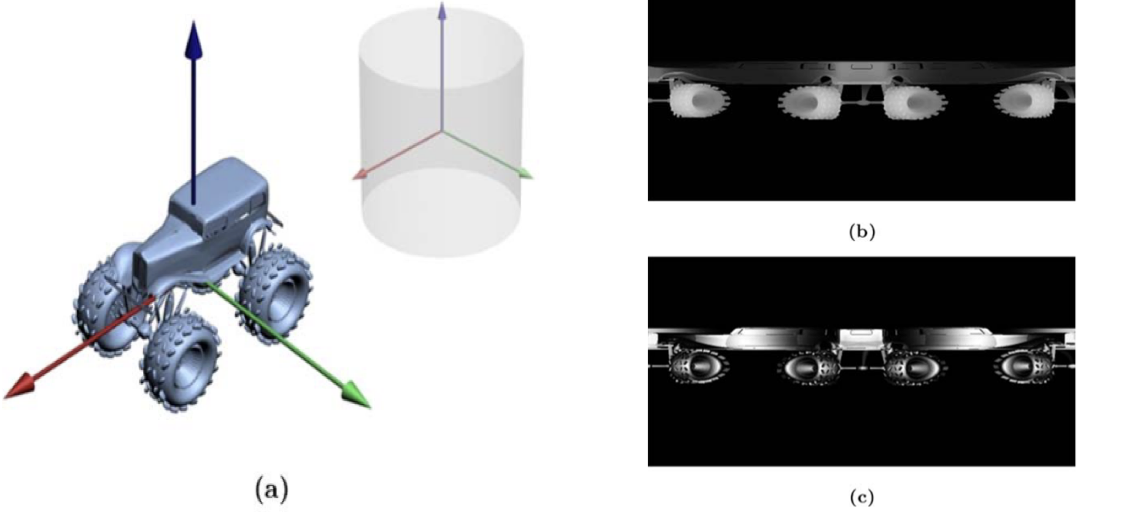
\includegraphics[width=1.0\linewidth]{image2.png}
    \caption{(a)Pose normalized 3D model, (b)the unfolded cylindrical projection of the 3D model capturing the position of the surface(the unfolded cylindrical projection of the 3D model capturing the orientation of the surface.)\cite{panorama}}
    \label{fig:method2}
\end{figure}

\textbf{Feature-based 3D protein alignment} is the method that we implement also in our approach. The method focuses on building a feature vector for each residue of each protein and that comparing the residues to one another, with methods like in our case the hungarian algorithm. 

\subsection{Protein structure comparison methods}
We take a deep dive in some frequently used methods such as 3D-Surfer, PANORAMA, DeepAlign, TM-Align. We take a look at some benchmarks presented by Figure ~\ref{fig:map_scores} and understand which method would be the best to compare two proteins. The explanation of each method will be provided below.\cite{shape}

The graph shows which method is better using benchmark levels such as: protein, species, and domain. 

\textbf{Protein} measures how well a shape matching method can compare the whole protein structure\cite{shape}. 

\textbf{Species} estimates whether proteins are correctly grouped according to the organism they come from, capturing evolutionary relationships within the same species\cite{shape}.

\textbf{Domain} benchmark test tests the performance of these methods across forms of life with very distant evolutionary relationships, making it the most challenging\cite{shape}.

In order to understand the graph, an explanation of the methods is required.

\textbf{3D-Surfer} is a method, where the global surface information of a protein is represented using 3D Zernike Descriptors(3DZD). These descriptors are moment-based invariants. The surface of a protein is triangulated and mapped into a 3D grid. From the mapping the 3DZD descriptors are calculated for the respective proteins. The Euclidean distance between two descriptors is used in order to assert the similarity between proteins.\cite{shape} 

\textbf{PANORAMA} is a shape retrieval method based on molecular surface maps. The explanation is provided above.

\textbf{DeepAlign} is a method that uses both sequence and structural alignment to find similarities between proteins, while also using deep learning. What it uses in order to find similarities are evolutionary relationships and hydrogen-bonding similarity.\cite{shape}

\textbf{TM-Align} generates residue-to-residue alignment based on structural similarity between protein pairs independently of their sequences using heuristic dynamic programming. The scoring function is called TM-score, and the method tries to maximise it.\cite{shape}

All in all the graph compares the performance of different structural alignment and shape retrieval methods (3D-Surfer, PANORAMA, DeepAlign, TM-Align) across three benchmark levels: protein, species, and domain. Explanation of each is provided above. Moreover, it shows how well each method captures similarities at the fine-grained protein level, the evolutionary grouping at the species level, and the broad classification at the domain level. Therefore this makes it possible for the most accurate method overall to be distinguished.

\section{Methods}
\subsection{PDB Files}
Figure ~\ref{fig:lol} shows how a snippet from a PDB file would look like in VS Code.

As stated above, every protein is given as PDB file, which captures every feature of the protein. The key elements of a PDB file would be:

\begin{figure}
    \centering
    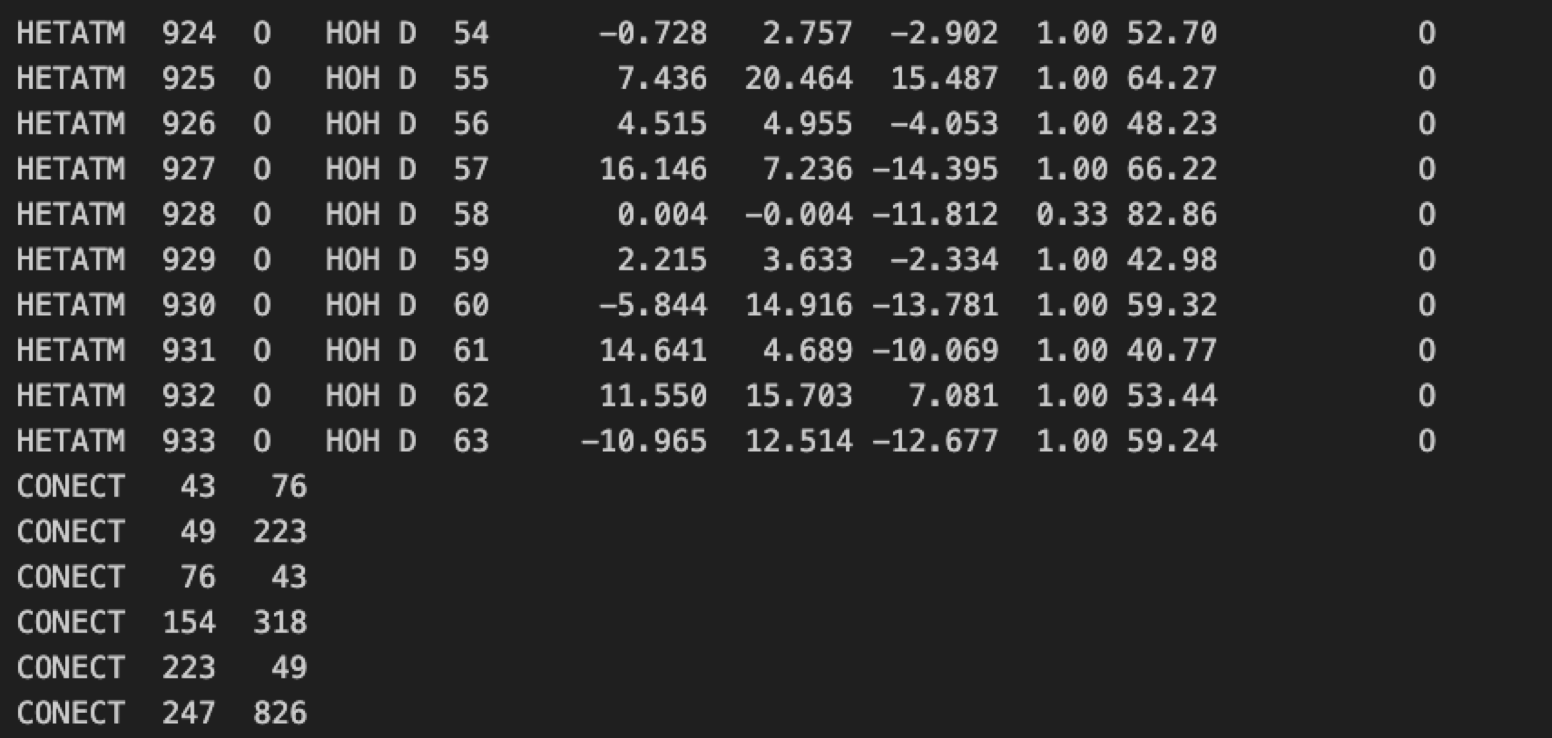
\includegraphics[width=1.0\linewidth]{image4.png}
    \caption{Example snippet from a PDB file.}
    \label{fig:lol}
\end{figure}

\textbf{1.HEADER} provides the name of the protein, classification, deposition date, and PDB ID\cite{brasier_pdb_medium}.

\textbf{2.TITLE} contains the protein's function, relevant experimental conditions, and provides a general description of what the PDB file contains\cite{brasier_pdb_medium}.

\textbf{3.COMPND} describes the macromolecular components of the structure\cite{brasier_pdb_medium}.

\textbf{4.AUTHOR} lists all the names of the researches that submitted the PDB file\cite{brasier_pdb_medium}.

\textbf{5.ATOM} is the section of the PDB file that contains the coordinates of each atom in the macromollecule. It also contains the name of each atom, residue name, chain id , residue number and also occupancy.\cite{brasier_pdb_medium}

\textbf{6.HETATM} records in a PDB file describe non-standard atoms such as ligands, cofactors, ions, or water molecules\cite{brasier_pdb_medium}. Ligands are small molecules that bind to proteins, cofactors are non-protein compounds that assist enzyme activity, and ions are charged atoms or molecules that stabilize structures or support biological processes.

\textbf{7.HELIX AND SHEET} gives information on secondary structures like alpha-helixes and beta-helixes, specifying even further the residues involved\cite{brasier_pdb_medium}. Alpha-helices are spiral-shaped structures in proteins stabilized by hydrogen bonds, while beta-sheets (often called beta-helices in general talk) are sheet-like structures formed by hydrogen bonding between aligned strands\cite{alpha_beta}. Hydrogen bonding are bonds that arise due to interaction between a hydrogen atom that is bonded to two highly electronegative atoms\cite{h_bonding}.

\textbf{8.CONECT} lists the connectivity information in the protein structure such as covalent and non-covalent bonds, includign disulfide bridges\cite{brasier_pdb_medium}. Figure ~\ref{fig:placeholder4} shows how a dislufite brige looke like. As seen from the figure ~\ref{fig:placeholder4} each protein contains a sulphur atom that pull each other and therefore the bond is created.

\begin{figure}
    \centering
    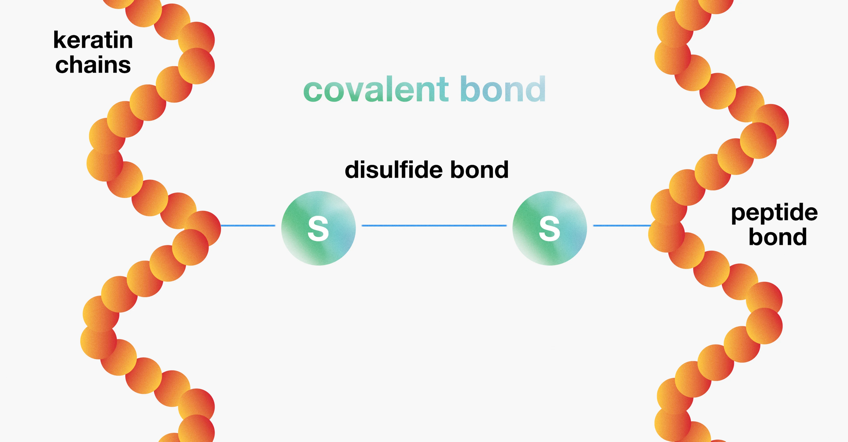
\includegraphics[width=1.0\linewidth]{image5.png}
    \caption{Disulfide bonds\cite{ds_bond}}
    \label{fig:placeholder4}
\end{figure}

\subsection{PDB Files Used in This Project}
Each PDB file that we work with is found on these links below:

\textbf{3nir.pdb (Pig insulin):} \url{https://www.rcsb.org/structure/1ZNI} \cite{pdb_1zni}

\textbf{4nir.pdb (Human insulin):} \url{https://www.rcsb.org/structure/3I40}\cite{pdb_3i40}
\begin{figure*}[t!]
  \centering
  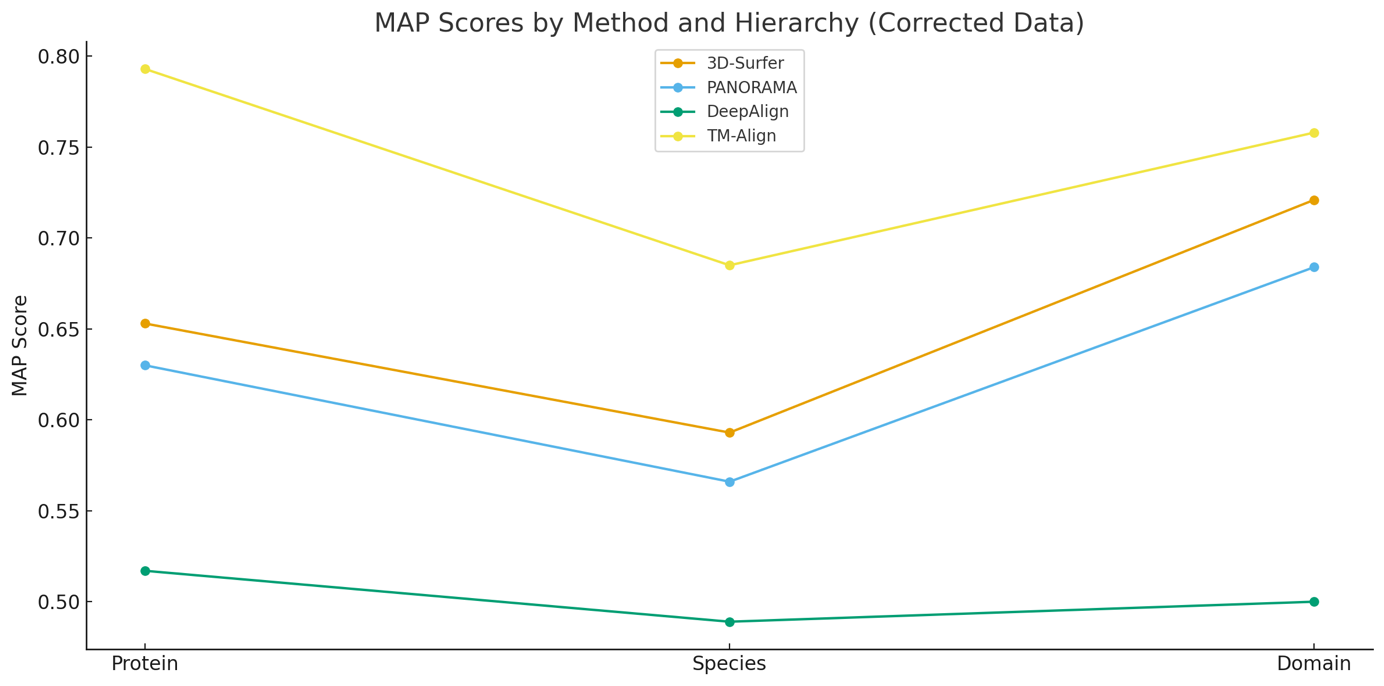
\includegraphics[width=0.75\textwidth]{image3.png}
  \caption{MAP Scores by Method and Hierarchy (corrected data). The figure compares the performance of different structural alignment and shape retrieval methods (3D-Surfer, PANORAMA, DeepAlign, TM-Align) across three levels: protein, species, and domain.}
  \label{fig:map_scores}
\end{figure*}
\subsection{PDB File Parsing and Graph Construction}
With the help of the article \cite{brasier_pdb_medium} we were able to produce code and therefore extract the coordinates of the individual atoms in each PDB file and render how would a protein look like. The code helps us also extract the C$\alpha$ (alpha carbon) coordinates in order for us to create nodes that represent the amino acids, bonded together with peptide bonds. We use the C$\alpha$ as a reference for every amino acid. Each molecule contains a central carbon (C) atom, called the $\alpha$-carbon, to which both an amino and a carboxyl group are attached. Figure~\ref{fig:alanine} shows each group. Each amino acid contains only one $\alpha$-carbon to the centre therefore we take it a point of reference to visualize each amino acid. 

We show in \url{3D_Shape_Matching_Ernald_Shehaj}\cite{shehaj2025} in the method called \url{protein_pdb_methods.py} we show how to render each atom part of the protein and also how to build a graph that represents amino acids as nodes and the peptide bonds as edges.

\textbf{1.\url{read_pdb_to_dataframe}.}The first step of our workflow involves parsing Protein Data Bank (PDB) files into a format that can be easily processed and analysed and for this purpose, we use the \url{read_pdb_to_dataframe} function, which leverages the BioPandas library. A Panda DataFrame is created by reading and converting the contents of a PDB file, which provides a structured representation of the atomic information. Features of the PDB file such as atom coordinates, residue names, chain identifiers, and element symbols get converted to build the DataFrame. The function also extracts header metadata from the file, which provides useful contextual information about the protein, such as methods, classification, and biological annotations. 

After the function loads the PDB file into a Pandas DataFrame, the DataFrame is further processes with the help of \url{process_dataframe} function in our code. The function of this method nothing more than to clean up the DataFrame. Alternate atom locations(alt\_loc) get resolved and the structure(DataFrame) is filtered based on the wanted level of granularity. By the selection of C$\alpha$ as the level of granularity, we can serve a reduced representation of the protein backbone. Each residue (amino acid) is then assigned a unique node identifier using the \url{label_node_id} from the Graphein library. This ensures that the protein's structure can be later modelled as a graph. 

\textbf{2.\url{Graph_construction}.} In Figure~\ref{fig:backbone} a clear visualization of the pig insulin as a graph. 
\begin{figure}
    \centering
    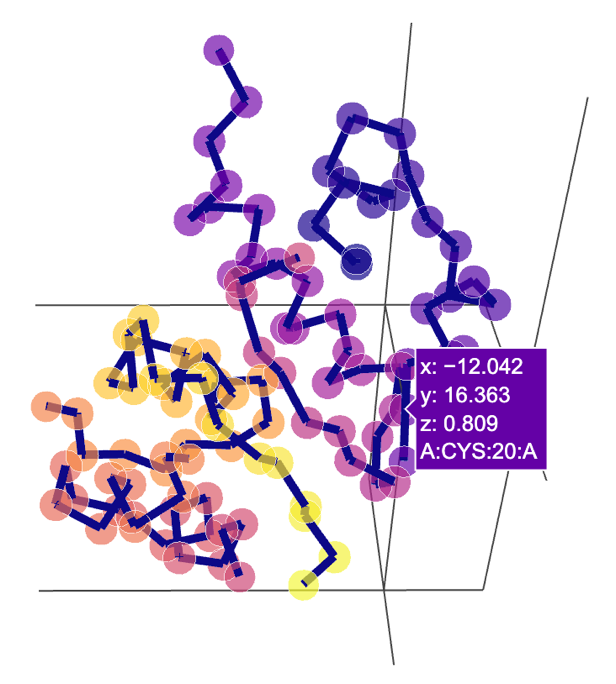
\includegraphics[width=1.0\linewidth]{image6.png}
    \caption{Backbone Protein Graph}
    \label{fig:backbone}
\end{figure}
Each amino acid is treated as a node, and the connections between them are represented as edges. The \url{add_backbone_edges} function links the nodes sequentially. The function that we implemented works in the way that it sorts the residues in order of their residue number, which is contained in the PDB file, and adds edges between consecutive residues, which are called backbone bonds. In this visualization, the nodes that belong to the same chain are coloured the same. A protein is made of chains of amino acids, where in our case here we have chain A, B, C, and D of the pig insulin. Chain A for example is coloured violet. \url{Build_backbone_graph} is the function that creates the residue-level graph using the Graphein library. The graph is initialized with the chain identifier, then it adds nodes that represent residues from the DataFrame. The backbone edges are attached after in order to reflect the protein's structural sequence. Lastly, the \url{visualize_backbone_graph} function uses \textbf{Plotly} to generate a 3D interactive visualization of the graph. 

\textbf{3.\url{Atom_level_plotting}.}In Figure~\ref{fig:atom} a clear visualization of the pig insulin as a plotting of atoms. 
\begin{figure}
    \centering
    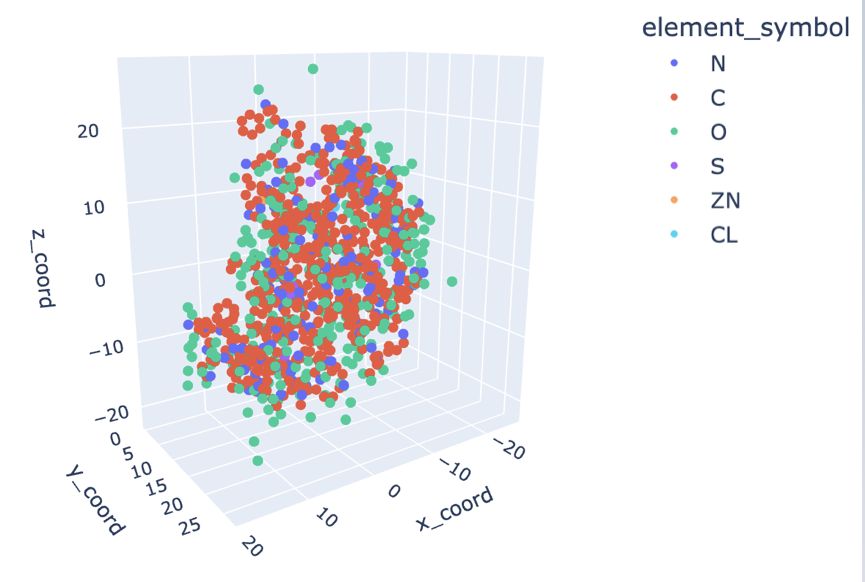
\includegraphics[width=1.0\linewidth]{image7.png}
    \caption{Plotted Atoms of the Pig Insulin}
    \label{fig:atom}
\end{figure}
The function \url{plot_atoms_with_bonds} creates an interactive 3D visualization of all atoms that are included in the PDB File. The function draws atoms as 3D markers by using their Cartesian coordinates(x\_coord, y\_coord, z\_coord). The colouring is done by the \url{color_by} argument. This argument uses the argument \url{element_symbol} in order so that the elements part of the protein, which can be C, N, O, S appear with distinct, consistent colours.
\textbf{4.\url{plot_two_chains_with_interface}} is the final function on our \url{protein_pdb_methods.py} implementation. Figure~\ref{fig:atom_to_atom} provides a view of the interaction between two chains of amino acids. 
\begin{figure}
    \centering
    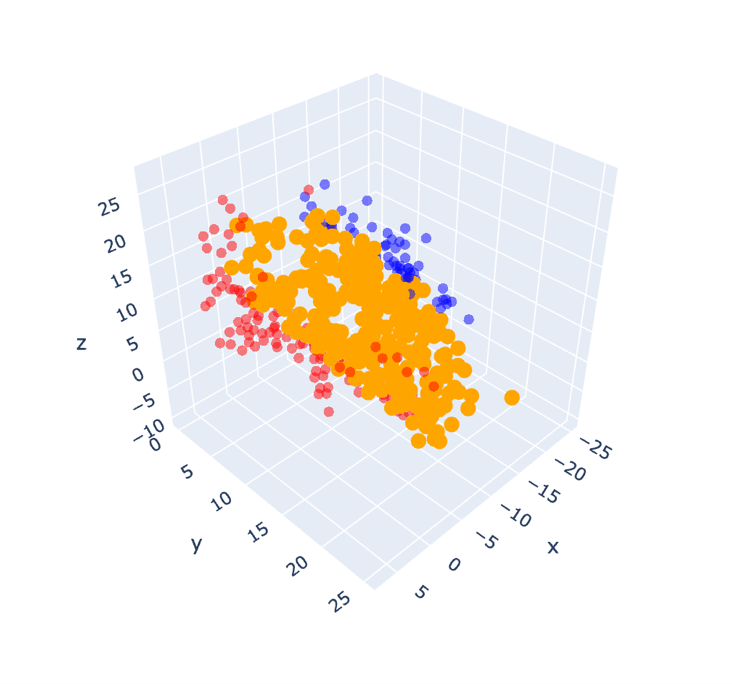
\includegraphics[width=1\linewidth]{image8.png}
    \caption{1) Chain A (Blue), 2) Chain B (Red), 3) Contact Atoms (Yellow).}
    \label{fig:atom_to_atom}
\end{figure}
Chain A is shown in blue and Chain B in red. This function tries to highlight interaction between two chains by detecting and displaying in orange spatially close atoms. \url{plot_two_chains_with_interface} checks for atoms that are within a threshold distance of 7.0 7.0~\AA\footnote{\AA{} (ångström) is a unit of length commonly used in molecular biology and structural chemistry, equal to $10^{-10}$ meters\cite{britannica_angstrom}.} from one another across the two chains. These contact atoms, can indicate points such as hydrogen bonding. 
\subsection{Feature-based 3D protein alignment}
In this section, we will talk about how we take two proteins and compare them using the Hungarian algorithm. How we build feature vectors for each residue, and how we build the matrix that makes the matching using the Hungarian method possible. 
This work presents nothing more than a feature based approach, which compares protein structures through C$\alpha$(alpha-carbon) atom alignment. Figure~\ref{fig:hungarian} shows the visualization of the comparison between the human insulin\url{4nir.pdb} and the pig insulin\url{3nir.pdb}. 
\begin{figure*}[t!]
  \centering
  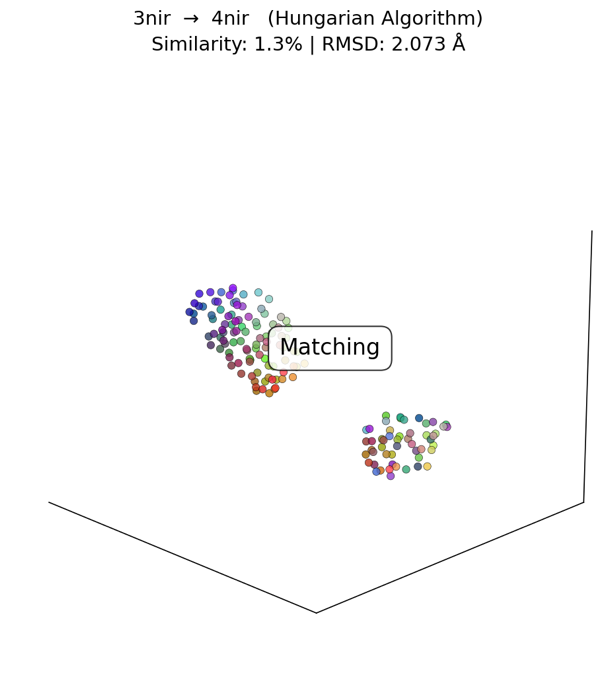
\includegraphics[width=0.5\textwidth]{image9.png}
  \caption{}
  \label{fig:hungarian}
\end{figure*}
\subsubsection{Core Components}
\textbf{k-Nearest Neighbors(kNN) Fingerprinting} is an algorithm that for each residue it computes the distance of each residue to its k nearest neighboring C$\alpha$ atoms, where typically the k=10(10 nearest neighbours). In order to find the distance between residue i and neighbours j, we computed the Euclidean distance:

d_{ij} = \sqrt{(x_i - x_j)^2 + (y_i - y_j)^2 + (z_i - z_j)^2}

The distances form a k-dimensional feature vector for each residue. 
When we build the cost matrix, the kNN cost, while trying to match residue i to j is calculated as the normalized Euclidean distance between their respective kNN vectors:

C_{knn}(i,j) = w_{knn} \times \frac{\|KNN_A(i) - KNN_B(j)\|_2}{k \times 10.0} 

This is the first step.\cite{cover1967nearest}

\textbf{Secondary Structure Prediction} with the usage of backbone angles tries to find the secondary structures. 
$$\theta = \arccos(\mathbf{u} \cdot \mathbf{v}), \text{ where } \mathbf{u} = \frac{\mathbf{p}_1 - \mathbf{p}_2}{\|\mathbf{p}_1 - \mathbf{p}_2\|} \text{ and } \mathbf{v} = \frac{\mathbf{p}_3 - \mathbf{p}_2}{\|\mathbf{p}_3 - \mathbf{p}_2\|}$$
where $\mathbf{p}_i = [x_i, y_i, z_i]$, finds the angle between three consecutive alpha-Carbon molecules.

$$\phi = \text{atan2}(y, x), \text{ where } x = \mathbf{v} \cdot \mathbf{w} \text{ and } y = (\mathbf{b}_1 \times \mathbf{v}) \cdot \mathbf{w}$$
gives the dihedral angle between 4 consecutive C$_\alpha$ carbons with $\mathbf{b}_0 = \mathbf{p}_2 - \mathbf{p}_1$, $\mathbf{b}_1 = \mathbf{p}_3 - \mathbf{p}_2$, $\mathbf{b}_2 = \mathbf{p}_4 - \mathbf{p}_3$, and $\mathbf{v}$, $\mathbf{w}$ being projections perpendicular to $\mathbf{b}_1$. Helices are identified by $80° \leq \theta \leq 120°$ and $-90° \leq \phi \leq -30°$, while beta sheets show $100° \leq \theta \leq 140°$ and $|\phi| \geq 160°$\cite{delacruz1997discrete,flocco1995c,keskin1998packing,grassein2020curvature,wikipedia2025dihedral,korkut2009force}.

\textbf{Residue Chemistry Classification} Each amino acid is part of a chemical category. \cite{shehaj2025} the code of the project in the \url{compare_pdb_rmsd.py} it is shown that amino acids can be hydrophobic, aromatic, polar, negatively charged, and positively charged\cite{taylor1986}. The cost matrix works in the way such as if we have identical chemistry between residues we have zero cost, same broad category receives 0.4, and different categories receive 1.0. This ensures chemical sensible correspondences.  

\textbf{Kabsch Algorithm} is used in order to produce rotation invariance, computing the optimal matrix \textbf{R} and translation vector \textbf{t} that minimises the RMSD between two point sets P and Q in 3Dspace, following the steps\cite{kabsch}:
\begin{itemize}
    \item Compute centroids of $\mathbf{P}$ and $\mathbf{Q}$
    \item Center both point sets by subtracting centroids
    \item Compute cross-covariance matrix $\mathbf{C} = \mathbf{P}'^T \mathbf{Q}'$
    \item Compute SVD: $\mathbf{C} = \mathbf{U} \mathbf{\Sigma} \mathbf{V}^T$
    \item Compute $d = \text{sign}(\det(\mathbf{V} \mathbf{U}^T))$ and $\mathbf{B} = \text{diag}(1, 1, d)$
    \item Optimal rotation: $\mathbf{R}^* = \mathbf{V} \mathbf{B} \mathbf{U}^T$
    \item Optimal translation: $\mathbf{t}^* = \bar{\mathbf{q}} - \bar{\mathbf{p}}$
\end{itemize}

The RMSD between aligned point sets is\cite{kabsch}:
$$\text{RMSD} = \sqrt{\frac{1}{N} \sum_{i=1}^{N} \|\mathbf{q}_i - \mathbf{R}^*(\mathbf{p}_i + \mathbf{t}^*)\|^2}$$
\subsubsection{Alignment Pipleline}
The cost matrix is formed on this way:

C(i,j) = w_{knn} \times C_{knn} + w_{ss} \times C_{ss} + w_{chem} \times C_{chem} + w_{rmsd} \times C_{rmsd}

The Hungarian algorithm produces an initial matching without using Kabsch alignment and then the whole alignment is repeated when we do use Kabsch to align the residues. After alignment, poorly matched pairs with distance above 3.5 Å are removed. The similarity score combines coverage and fit quality:
$$\text{Similarity} = 100 \times \frac{\text{kept\_pairs}}{\min(N_A, N_B)} \times \frac{1}{1 + \alpha \times \text{RMSD}}$$
The output includes a CSV mapping. The CSV mapping gets visualized in \url{visualize_match.py}.

\section{Discussion}
The method talked above can indeed generate a matching between proteins, but it has many flaws. Firstly, it does not check if the residues are of the same type, but it rather concentrates in their position in the 3D space. Moreover, it is not very able in error handling. If a protein has a missing residue, the algorithm here cannot skip them. Instead, it forces a one to one match. The method implemented by us is also very sensitive to noise, where a few outlier residues with bad coordinates can distort the match and affect the RMSD. Lastly, the Hungarian algorithm method is a greedy matching method that sometimes cannot implement methods that may be biologically more meaningful. 
\section{Conclusions}
However, the code is able to perform very well on feature based comparison. It takes into consideration features that we discussed above in order to find the best matching. The usage of the Kabsch Algorithm brought rotation invariance, where it removes translation/rotation effects. In this case, we also saw that the code was able to work with different sizes of proteins, like the pig insulin and the human insulin, which have different sizes. Lastly, the code provides at the end similarity scoring and a visual output. 

\section{Code availability}
The code developed for this report can be found in the repository provided with the report:
3D_Shape_Matching_Ernald_Shehaj

\printbibliography
\end{document}